\section{Proof the Theorem}
$(\Rightarrow)$  Nếu đồ thị $G$ chứa đồ thị con là subdivision của $K_5$ hoặc $K_{3,3}$ thì $G$ không phẳng. \\

\begin{proof}
    Ta có:
    \begin{itemize}
        \item Subdivision của đồ thị không phẳng thì không phẳng

        \item Nếu một đồ thị con không phẳng thì đồ thị không phẳng

        \item Nếu một đồ thị con của đồ thị $G$ là subdivision của đồ thị không phẳng thì $G$ không phẳng
    \end{itemize}
    \begin{lemma}
        $K_{3,3}$ is không phẳng
    \end{lemma}

    \begin{proof}
        Chúng ta sẽ chứng minh bằng phản chứng.

        Giả sử tồn tại một biểu diễn phẳng của $K_{3,3}$. Trong đồ thị phân đôi đơn, chiều dài nhỏ nhất của chu trình là 4, nghĩa là với mọi $f \in F(K_{3,3})$
        $$deg(f) \geq 4$$
        Lại có $$\sum_{f \in F(K_{3,3})}deg(f) = 2\epsilon$$
        \begin{figure}[H]
            \begin{minipage}{0.3\textwidth}
                $$V-E+F=2$$
                $$6-E+F=2$$
                $$6-9+F=2$$
                $$F=5$$
            \end{minipage}
            \hfill
            \begin{minipage}{0.35\textwidth}
                \centering
                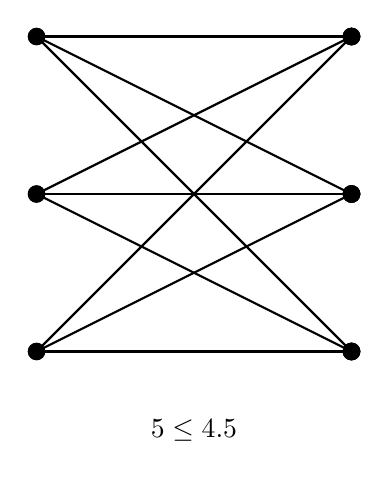
\begin{tikzpicture}
                    \foreach \x/\y in {0/1, 0/3, 0/5} {
                            \filldraw[black] (\x,\y) circle (3pt);
                            \foreach \z/\t in {4/1, 4/3, 4/5} {
                                    \filldraw[black] (\z,\t) circle (3pt);
                                    \draw[black, thick] (\x,\y) -- (\z,\t);
                                }
                        }
                    \node at (2,0,0) {$5 \leq 4.5$};
                \end{tikzpicture}
            \end{minipage}
            \hfill
            \begin{minipage}{0.3\textwidth}
                \centering
                % No 3 edge faces
                $$4F \leq 2E$$
                $$4F \leq 2 \times 9$$
                $$ F \leq 4.5$$
            \end{minipage}
        \end{figure}
    \end{proof}

    \begin{lemma}
        $K_5$ is không phẳng
    \end{lemma}
    \begin{proof}
        Giả sử tồn tại một biểu diễn phẳng của $K_{3,3}$. Trong đồ thị phân đôi đơn, chiều dài nhỏ nhất của chu trình là 4, nghĩa là với mọi $f \in F(K_{3,3})$
        $$deg(f) \geq 3$$
        Lại có $$\sum_{f \in F(K_{3,3})}deg(f) = 2\epsilon$$
        \begin{figure}[H]
            \begin{minipage}{0.3\textwidth}
                $$V-E+F=2$$
                $$5-E+F=2$$
                $$5-10+F=2$$
                $$F=7$$
            \end{minipage}
            \hfill
            \begin{minipage}{0.35\textwidth}
                \centering
                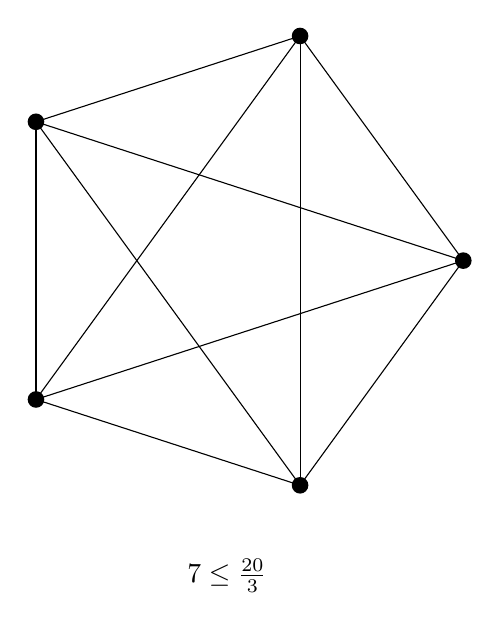
\begin{tikzpicture}
                    \foreach \i in {1, 2, 3, 4, 5}
                    \fill[black] (\i*360/5:3) coordinate (5\i) circle(3 pt)
                    \ifnum \i>1 foreach \j in {\i,...,1}{(5\i) edge (5\j)} \fi;

                    \node at (0,-4,0) {$7 \leq \frac{20}{3}$};
                \end{tikzpicture}
            \end{minipage}
            \hfill
            \begin{minipage}{0.3\textwidth}
                \centering
                $$3F \leq 2E$$
                $$3F \leq 2 \times 10$$
                $$F \leq \frac{20}{3}$$
            \end{minipage}
        \end{figure}
    \end{proof}
    \begin{recap}
    \end{recap}
    $K_5$ và $K_{3,3}$ là không phẳng

    $\Rightarrow$ Tất cả subdivisions của chúng đều không phẳng

    $\Rightarrow$ Nếu đồ thị $G$ chứa đồ thị con là subdivision của $K_5$ hoặc $K_{3,3}$ thì G không phẳng \\

\end{proof}
$(\Leftarrow)$ Nếu đồ thị $G$ không phẳng thì $G$ chứa subdivision của $K_5$ hoặc $K_{3,3}$
\begin{proof}
    Giả sử tồn tại đồ thị không phẳng mà không chứa đồ thị con là subdivisions của $K_5$ hoặc $K_{3,3}$.

    Cho $G$ là đồ thị có \textit{ít cạnh nhất}. Khi loại bỏ một cạnh bất kì của $G$ thì ta được đồ thị \textit{phẳng}.

    \begin{enumerate}
        \item $G$ là 2-connected
              \begin{proof}
                  \begin{figure}[H]
                      \centering
                      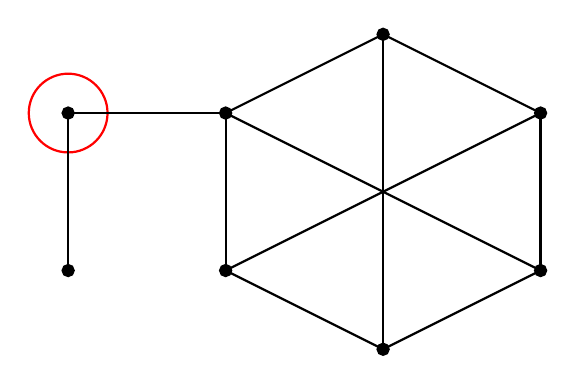
\begin{tikzpicture}
                          \draw[red, thick] (-2,3) circle (0.5);
                          \foreach \x/\y in {0/1, 2/0, 4/1, 0/3, 4/3, 2/4} {
                                  \filldraw[black, thick] (\x,\y) circle (2pt);
                                  \draw[black, thick] (2,2) -- (\x,\y);
                              }
                          \filldraw[black, thick] (-2,3) circle (2pt);
                          \filldraw[black, thick] (-2,1) circle (2pt);

                          \draw[black, thick] (0,1) -- (2,0);
                          \draw[black, thick] (2,0) -- (4,1);
                          \draw[black, thick] (4,1) -- (4,3);
                          \draw[black, thick] (0,3) -- (0,1);
                          \draw[black, thick] (4,3) -- (2,4);
                          \draw[black, thick] (2,4) -- (0,3);

                          \draw[black, thick] (-2,1) -- (-2,3);
                          \draw[black, thick] (-2,3) -- (0,3);

                      \end{tikzpicture}
                  \end{figure}
                  Đầu tiên, ta chỉ ra $G$ 1-connected (liên thông). Giả sử $G$ không liên thông, và không phẳng.
                  Vì $G$ là đồ thị không phẳng \textit{ít cạnh nhất} nên các thành phần của nó là phẳng. Không mất tính tổng quát, giả sử G có 2 thành phần liên thông là $G_1$ và $G_2$.
                  Bởi vì $G_1$ và $G_2$ cùng phẳng, ta có thể thêm biểu diễn phẳng của $G_1$ vào một trong các diện biểu diễn phẳng của $G_2$ (ví dụ diện vô hạn), cho ta biểu diễn phẳng của $G$. Vô lý.

                  Vì $G$ liên thông nên $\kappa(G) \geq 1$. Giả sử $\kappa(G) = 1$, theo định nghĩa, tồn tại đỉnh $v$ sao cho $G -v$ không liên thông.
                  Không mất tính tổng quát, giả sử $G-v$ có 2 thành phần liên thông $H_1$ và $H_2$.
                  Ta có $H_1 \cup v$ và $H_2 \cup v$ đều phẳng vì tính cực tiểu của $G$.
                  Trong biểu diễn phẳng của chúng, ta có thể tìm một diện $f$ mà biên chứa đỉnh $v$.
                  Với phép chiếu lập thể, ta có thể thu được biểu diễn phẳng của $H_1 \cup v$ và $H_2 \cup v$ mà $v$ nằm trên đường biên của diện không bị chặn.
                  Bằng cách đặt điểm ở vô cùng.
                  Sau đó, ta gộp $H_1 \cup v$ và $H_2 \cup v$ bằng cách hợp nhất $v$ và thu được một biểu diễn phẳng của G. Vô lý.

                  Vậy, nếu $G$ là đồ thị không phẳng cực tiểu thì $G$ 2-connected.

              \end{proof}

        \item Nếu $G$ là đồ thị không phẳng \textit{ít cạnh nhất} và $xy$ là một cạnh của $G$ thì $G-xy$ 2-connected
              \begin{proof}
                  Vì $G$ 2-connected nên $\kappa(G) \geq 2$. Giả sử $\kappa(G) =2$ thì tồn tại 2 đỉnh $u,v$ sao cho $G-\{u,v\}$ không liên thông.
                  Gọi các thành phần liên thông của $G-\{u,v\}$ là $H_1, H_2, \ldots,H_k$. Xây dựng tập $M_1,M_2,\ldots,M_k$ trọng đó $M_i=H_i \cup \{u,v\} +uv$.
                  Ta sẽ chỉ ra tồn tại $M_i (1 \geq i \geq k)$ không phẳng.

                  Giả sử tất cả $M_i (1 \geq i \geq k)$ đều phẳng, do đó tồn tại biểu diễn phẳng của mỗi chúng. Với phép chiếu lập thể, ta luôn có một biểu phẳng sao cho $uv$ là biên của diện vô hạn.
                  Vì $\{u,v\}$ và $uv$ là phân chung duy nhất của các $M_i$, do đó, ta có thể hợp nhất biểu diễn phẳng của chúng, thu được biểu diễn phẳng của $G+uv$.
                  Nghĩa là $G+uv$ phẳng, nên $G$ cũng phẳng. Vô lý, do đó tồn tại $M_j (1 \geq j \geq k)$ không phẳng.

                  Giả sử $H_p (1 \geq p \geq k)$ là một thành phần liên thông của $G$.
                  Nếu trong 2 đỉnh $u,v$ không có đỉnh nào nổi với $H_p$, khi đó, $H_p$ là một thành phần liên thông, hay $G$ không liên thông, vô lý.
                  Nếu trong 2 đỉnh $u,v$ có một đỉnh nối tới $H_p$, giả sử $u$, thì khi xóa đỉnh $u$, $G-u$ không còn liên thông, hay $\kappa(G)=1$, vô lý.
                  Vậy cả $u$ và $v$ đều có cạnh nối tới $H_p$ hay có ít nhất 2 cạnh từ $\{u,v\}$ nối đến $H_p$

                  Ta có:
                  \begin{eqnarray*}
                      \epsilon(G)& \geq &\epsilon(H_j+\{u,v\}) + \epsilon(H_p +\{u,v\}) \\
                      & \geq & \epsilon(H_j+\{u,v\}) + 2\\
                      & > & \epsilon(H_j+\{u,v\}) + 1 \\
                      & = & \epsilon(H_j+\{u,v\} + uv) = \epsilon(M_j)
                  \end{eqnarray*}
                  Cuối cùng thì $\epsilon(M_j) < \epsilon(G)$. Vì $G$ là đồ thị ít cạnh nhất không chứa subdivision $K_5$ và $K_{3,3}$, $M_j$ không phẳng và ít cạnh hơn $G$, nên $M_j$ phải chứa subdivision của $K_5$ hoặc $K_{3,3}$.
                  Suy ra $M_j$ không phải đồ thị con của $G$.
                  Lại có $M_j -uv$ là đồ thị con của $G$ nghĩa là $G$ không chứa cạnh $uv$.
                  Ta hợp nhất $M_j-uv$ với $M_p-uv$ bằng cách hợp nhất đỉnh $u$ và đỉnh $v$, ta thu được một đồ thị con của $G$.
                  Do $M_p -uv$ liên thông nên tồn tại một path giữa $u$ và $v$, kết hợp path này với $M_j-uv$ ta được một subdivision của  $K_5$ hoặc $K_{3,3}$.
                  \begin{figure}[H]
                      \centering
                      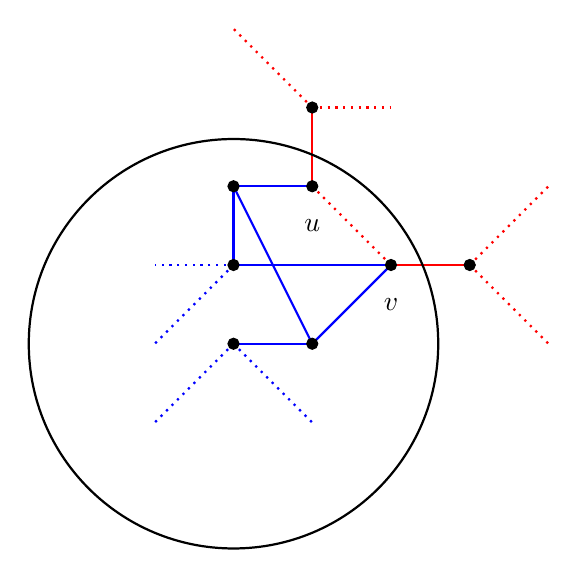
\begin{tikzpicture}
                          \node at (0,0.5,0){$u$};
                          \node at (1,-0.5,0){$v$};
                          \draw[blue, thick] (0, -1) -- (-1,1);
                          \draw[blue, thick] (-1, 0) -- (1,0);
                          \draw[blue, thick] (0, -1) -- (-1,-1);
                          \draw[blue, thick] (0, 1) -- (-1,1);
                          \draw[blue, thick] (-1, 0) -- (-1,1);
                          \draw[blue, thick] (1, 0) -- (0,-1);
                          \draw[red, thick] (1, 0) -- (2,0);
                          \draw[red, thick] (0, 1) -- (0,2);
                          \draw[black, thick] (-1,-1) circle (2.6);
                          \draw[dotted, red, thick] (0, 1) -- (1,0);
                          \draw[dotted, red, thick] (2, 0) -- (3,1);
                          \draw[dotted, red, thick] (2, 0) -- (3,-1);
                          \draw[dotted, red, thick] (0, 2) -- (1,2);
                          \draw[dotted, red, thick] (0, 2) -- (-1,3);
                          \draw[dotted, blue, thick] (-1, 0) -- (-2,0);
                          \draw[dotted, blue, thick] (-1, 0) -- (-2,-1);
                          \draw[dotted, blue, thick] (-1, -1) -- (-2,-2);
                          \draw[dotted, blue, thick] (-1, -1) -- (0,-2);
                          \filldraw[black] (-1,1) circle (2pt);
                          \filldraw[black] (0,-1) circle (2pt);
                          \filldraw[black] (0,1) circle (2pt);
                          \filldraw[black] (1,0) circle (2pt);
                          \filldraw[black] (2,0) circle (2pt);
                          \filldraw[black] (-1,0) circle (2pt);
                          \filldraw[black] (-1,-1) circle (2pt);
                          \filldraw[black] (0,2) circle (2pt);
                      \end{tikzpicture}
                      \caption*{\textcolor{blue}{Xanh}: $M_j-uv$ \\ \textcolor{red}{Đỏ}: $M_p-uv$}
                  \end{figure}


                  Dẫn đến $G$ chứa subdivision của $K_5$ hoặc $K_{3,3}$. Vô lý

                  $\Rightarrow \kappa(G) \geq 3$ hay $G$ 3-connected.
              \end{proof}
              Tiếp theo, ta sẽ chỉ ra với mọi cặp đỉnh $a,b \in V(G-xy)$, tồn tại một chu trình đi qua chúng.
              Ta sẽ chứng minh qua 3 trường hợp.
              \begin{itemize}
                  \item $\{a,b\} = \{x,y\}$. Rõ ràng $\nu(G) \geq 4$ ?? :D ??. Chọn bừa 2 đỉnh $c$ và $d$ trong đồ thị $G-xy$.
                        Không mất tính tổng quát, giả sử $a=x$. Vì $G$ 3-connected nên loại bỏ 2 đỉnh không làm mất tính liên thông của $G$.
                        nghĩa là khi loại bỏ $y$ và $d$, vẫn còn một path nối giữa $x$ và $c$. Nói cách khác, có một path $P_1$ giữa $x$ và $c$ không đi qua $y$ và $d$.
                        Tương tự, có một path $P_2$ giữa $c$ và $y$ không đi qua $x$ và $d$,
                        một path $P_3$ giữa $y$ và $d$ không đi qua $x$ và $c$,
                        một path $P_4$ giữa $d$ và $x$ không đi qua $y$ và $c$.
                        Khi đó, ta có $x$ và $y$ cùng nằm trên một chu trình $x-P_1-c-P_2-y-P_3-d-P_4-x$.
                  \item Có duy nhất 1 đỉnh trong $\{a,b\}$ là $x$ hoặc $y$. Không mất tính tổng quát, giả sử $a=x$ và $b \neq y$.
                        Chọn bừa 1 điểm $c \neq b$ không trùng $x$ và $y$. Tương tự trường hợp trên,
                        tồn tại một path $P_1$ giữa $x$ và $b$ không đi qua $c$ và $y$,
                        một path $P_2$ giữa $c$ và $b$ không đi qua $x$ và $y$,
                        một path $P_2$ giữa $c$ và $x$ không đi qua $x$. Ta lại thu được một chu trình $x-P_1-b-P_2-c-P_3-x$, chu trình này chứa cả $x$ và $b$.
                  \item Cả $a,b$ đều không trùng $x,y$. Lại một lần nữa, tương tự trường hợp trên,
                        tồn tại một path $P_1$ giữa $a,b$ không đi qua $x,y$,
                        một path $P_2$ giữa $b,y$ không đi qua $x,a$,
                        một path $P_1$ giữa $y,a$ không đi qua $x,b$. Ta thu được chu trình $a-P_1-b-P_2-y-P_3-a$ chứa cả $a$ và $b$.
              \end{itemize}
              Từ 3 trường hợp trên, luôn có một chu trình đi qua $a,b$ trong $G-xy$, nên $G-uv$ phải 2-connected.
              \begin{tikzpicture}

              \end{tikzpicture}
    \end{enumerate}


    Xét đồ thị $G-uv$ thu được bằng cách bỏ cạnh $uv$ từ $G$

    $G-uv$ là đồ thị phẳng

    $G-uv$ là 2-connected, nên tồn tại chu trình đi qua $u$ và $v$.

    \begin{remark}
        Chú ý những cạnh chúng tôi vẽ dưới đây là những path trong đồ thị.
    \end{remark}

    \begin{figure}[H]
        \begin{minipage}{0.4\textwidth}
            \begin{tikzpicture}
                \draw[black, thick] (0,0) circle (3);
                \filldraw[black, thick] (-3,0) circle (2pt);
                \filldraw[black, thick] (3,0) circle (2pt);
                \node at (-3.5,0,0) {$u$};
                \node at (3.5,0,0) {$v$};
                \node at (0,2.5,0) {$C$};
            \end{tikzpicture}
        \end{minipage}
        \hfill
        \begin{minipage}{0.5\textwidth}
            Gọi $C$ là chu trình dài nhất chứa $u,v$
        \end{minipage}

    \end{figure}

    \begin{figure}[H]
        \begin{minipage}{0.4\textwidth}
            \begin{tikzpicture}
                \draw[black, thick] (0,0) circle (3);
                \filldraw[black, thick] (-3,0) circle (2pt);
                \filldraw[black, thick] (3,0) circle (2pt);
                \node at (-3.5,0,0) {$u$};
                \node at (3.5,0,0) {$v$};
                \node at (0,2.5,0) {$C$};
            \end{tikzpicture}
        \end{minipage}
        \hfill
        \begin{minipage}{0.5\textwidth}
            Có một biểu diễn phẳng củ $G$ sao cho $C$ chiếm nhiều diện tích nhất trong tất cả các chu trình chứa $u$ và $v$
        \end{minipage}

    \end{figure}

    \begin{figure}[H]
        \begin{minipage}{0.4\textwidth}
            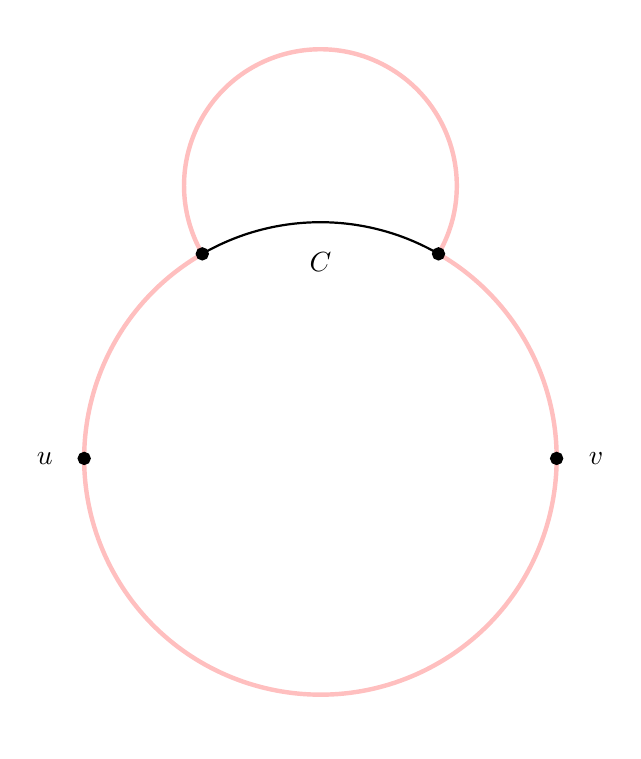
\begin{tikzpicture}
                \draw[pink, ultra thick] (1.5,{sqrt(27/4)}) arc (-30:210:{sqrt(3)});
                \draw[black, thick] (1.5,{sqrt(27/4)}) arc (60:120:3);
                \draw[pink, ultra thick] (-1.5,{sqrt(27/4)}) arc (120:420:3);
                \filldraw[black, thick] (1.5,{sqrt(27/4)}) circle (2pt);
                \filldraw[black, thick] (-1.5,{sqrt(27/4)}) circle (2pt);
                \filldraw[black, thick] (-3,0) circle (2pt);
                \filldraw[black, thick] (3,0) circle (2pt);

                \node at (-3.5,0,0) {$u$};
                \node at (3.5,0,0) {$v$};
                \node at (0,2.5,0) {$C$};
            \end{tikzpicture}
        \end{minipage}
        \hfill
        \begin{minipage}{0.4\textwidth}
            Ta không thể có extra paths ở phần trên hay dưới $C$ vì nó sẽ tạo ra chu trình chiếm nhiều diện tích hơn $C$, mâu thuẫn.
        \end{minipage}

    \end{figure}


    \begin{figure}[H]
        \begin{minipage}{0.4\textwidth}
            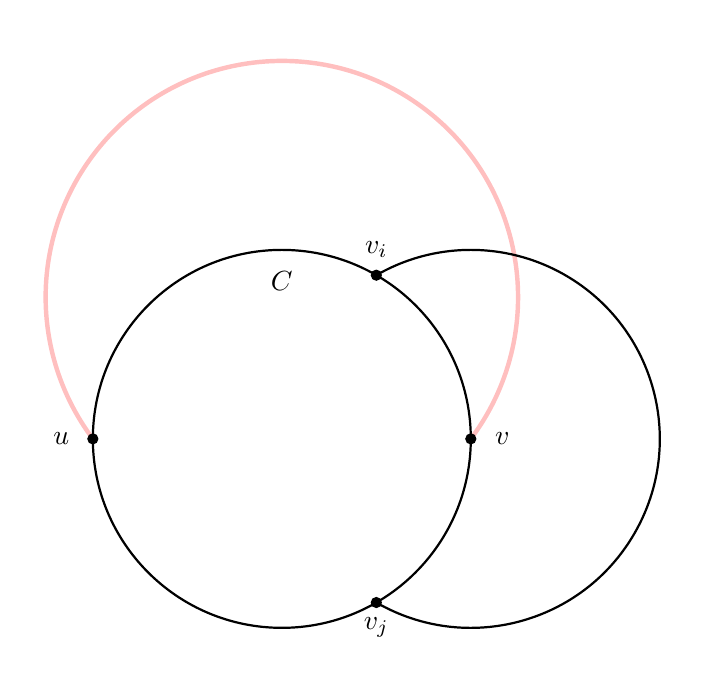
\begin{tikzpicture}[scale = 0.8]
                \draw[black, thick] (0,0) circle (3);
                \draw[pink, ultra thick] (3,0) arc (-acos(3/3.75):180+acos(3/3.75):3.75);
                \draw[black, thick] (1.5,-{sqrt(27/4)}) arc (-120:120:3);

                \filldraw[black, thick] (-3,0) circle (2pt);
                \filldraw[black, thick] (3,0) circle (2pt);
                \filldraw[black, thick] (1.5,{sqrt(27/4)}) circle (2pt);
                \filldraw[black, thick] (1.5,-{sqrt(27/4)}) circle (2pt);
                \node at (1.5,3,0) {$v_i$};
                \node at (1.5,-3,0) {$v_j$};
                \node at (-3.5,0,0) {$u$};
                \node at (3.5,0,0) {$v$};
                \node at (0,2.5,0) {$C$};
            \end{tikzpicture}
        \end{minipage}
        \hfill
        \begin{minipage}{0.4\textwidth}
            $G$ không phẳng, nên ta có một obstruction $uv$ ở phía ngoài của $C$. There must exist a path $v_iv_j$ that blocks $uv$
        \end{minipage}
    \end{figure}

    Phía trong của $C$ cũng cần có một obstruction. Cái obstruction này cũng phải block $v_iv_j$ và $uv$ from being draw inside of $C$ since otherwise we could just draw it inside and draw $uv$ on the outside.

    Tương đương, Ta có 4 loại obstructions tổng quát được miêu tả dưới đây. \\

    \begin{figure}[H]
        \begin{minipage}{0.4\textwidth}
            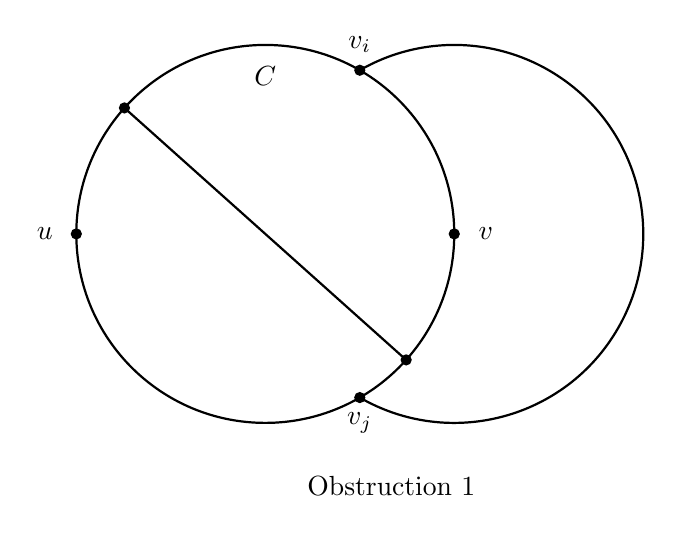
\begin{tikzpicture}[scale = 0.8]
                \draw[black, thick] (0,0) circle (3);
                \draw[black, thick] (1.5,-{sqrt(27/4)}) arc (-120:120:3);
                \draw[black, thick] ({-sqrt(5)},2) -- ({sqrt(5)},-2);
                \filldraw[black, thick] (-3,0) circle (2pt);
                \filldraw[black, thick] (3,0) circle (2pt);
                \filldraw[black, thick] ({-sqrt(5)},2) circle (2pt);
                \filldraw[black, thick] ({sqrt(5)},-2) circle (2pt);
                \filldraw[black, thick] (1.5,{sqrt(27/4)}) circle (2pt);
                \filldraw[black, thick] (1.5,-{sqrt(27/4)}) circle (2pt);
                \node at (1.5,3,0) {$v_i$};
                \node at (1.5,-3,0) {$v_j$};
                \node at (-3.5,0,0) {$u$};
                \node at (3.5,0,0) {$v$};
                \node at (0,2.5,0) {$C$};

                \node at (2,-4,0) {Obstruction 1};
            \end{tikzpicture}
        \end{minipage}
        \hfill
        \begin{minipage}{0.4\textwidth}
            \begin{tikzpicture}[scale = 0.8]
                \draw[black, thick] (0,0) circle (3);
                \draw[black, thick] (1.5,-{sqrt(27/4)}) arc (-120:120:3);
                \draw[black, thick] (3,0) arc (acos(0.6):180-acos(0.6):5);
                \draw[black, thick] ({sqrt(5)},-2) -- (-{sqrt(5)},2);
                \filldraw[blue, thick] (-3,0) circle (3pt);
                \filldraw[purple, thick] (3,0) circle (3pt);
                \filldraw[purple, thick] ({-sqrt(5)},2) circle (3pt);
                \filldraw[blue, thick] ({sqrt(5)},-2) circle (3pt);
                \filldraw[blue, thick] (1.5,{sqrt(27/4)}) circle (3pt);
                \filldraw[purple, thick] (1.5,-{sqrt(27/4)}) circle (3pt);
                \node at (1.5,3,0) {$v_i$};
                \node at (1.5,-3,0) {$v_j$};
                \node at (-3.5,0,0) {$u$};
                \node at (3.5,0,0) {$v$};
                \node at (0,2.5,0) {$C$};
                \node at (2,-4,0) {$G$ chứa một subdivision của $K_{3,3}$};

            \end{tikzpicture}
        \end{minipage}
    \end{figure}

    \begin{figure}[H]
        \begin{minipage}{0.4\textwidth}
            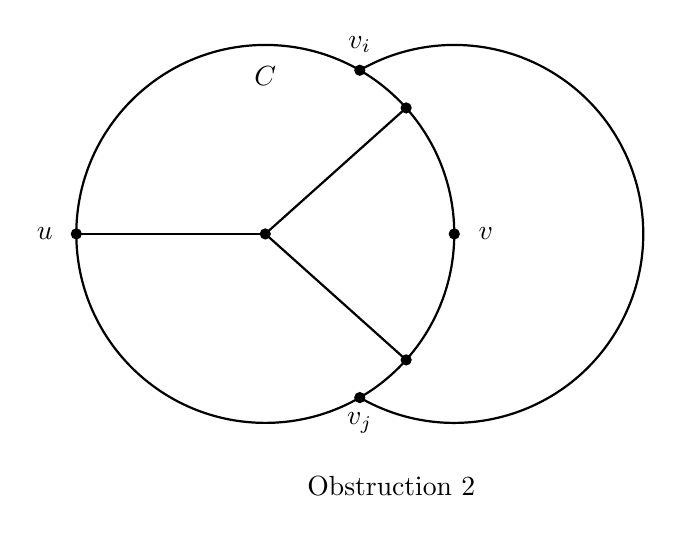
\begin{tikzpicture}[scale = 0.8]
                \draw[black, thick] (0,0) circle (3);
                \draw[black, thick] (1.5,-{sqrt(27/4)}) arc (-120:120:3);
                \draw[black, thick] (0,0) -- ({sqrt(5)},-2);
                \draw[black, thick] (0,0) -- ({sqrt(5)},2);
                \draw[black, thick] (0,0) -- (-3,0);
                \filldraw[black, thick] (-3,0) circle (2pt);
                \filldraw[black, thick] (3,0) circle (2pt);
                \filldraw[black, thick] (0,0) circle (2pt);
                \filldraw[black, thick] ({sqrt(5)},2) circle (2pt);
                \filldraw[black, thick] ({sqrt(5)},-2) circle (2pt);
                \filldraw[black, thick] (1.5,{sqrt(27/4)}) circle (2pt);
                \filldraw[black, thick] (1.5,-{sqrt(27/4)}) circle (2pt);
                \node at (1.5,3,0) {$v_i$};
                \node at (1.5,-3,0) {$v_j$};
                \node at (-3.5,0,0) {$u$};
                \node at (3.5,0,0) {$v$};
                \node at (0,2.5,0) {$C$};

                \node at (2,-4,0) {Obstruction 2};
            \end{tikzpicture}
        \end{minipage}
        \hfill
        \begin{minipage}{0.4\textwidth}
            \begin{tikzpicture}[scale = 0.8]
                \draw[black, thick] (0,0) circle (3);
                \draw[black, thick] (1.5,-{sqrt(27/4)}) arc (-120:120:3);
                \draw[black, thick] (3,0) arc (acos(0.6):180-acos(0.6):5);
                \draw[black, thick] (0,0) -- ({sqrt(5)},-2);
                \draw[black, thick] (0,0) -- ({sqrt(5)},2);
                \draw[black, thick] (0,0) -- (-3,0);
                \filldraw[blue, thick] (-3,0) circle (3pt);
                \filldraw[purple, thick] (3,0) circle (3pt);
                \filldraw[purple, thick] (0,0) circle (3pt);
                \filldraw[blue, thick] ({sqrt(5)},2) circle (3pt);
                \filldraw[blue, thick] ({sqrt(5)},-2) circle (3pt);
                \filldraw[black, thick] (1.5,{sqrt(27/4)}) circle (2pt);
                \filldraw[purple, thick] (1.5,-{sqrt(27/4)}) circle (3pt);
                \node at (1.5,3,0) {$v_i$};
                \node at (1.5,-3,0) {$v_j$};
                \node at (-3.5,0,0) {$u$};
                \node at (3.5,0,0) {$v$};
                \node at (0,2.5,0) {$C$};
                \node at (2,-4,0) {$G$ chứa một subdivision của $K_{3,3}$};

            \end{tikzpicture}
        \end{minipage}
    \end{figure}

    \begin{figure}[H]
        \begin{minipage}{0.4\textwidth}
            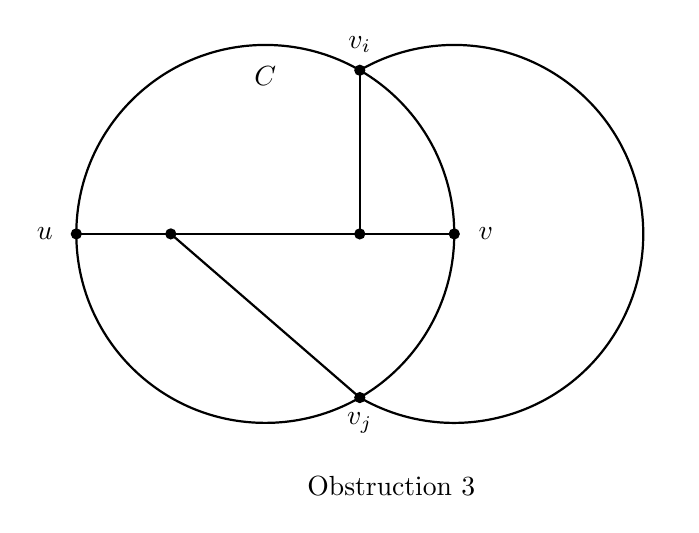
\begin{tikzpicture}[scale = 0.8]
                \draw[black, thick] (0,0) circle (3);
                \draw[black, thick] (1.5,-{sqrt(27/4)}) arc (-120:120:3);
                \draw[black, thick] (3,0) -- (-3,0);
                \draw[black, thick] (1.5,0) -- (1.5,{sqrt(27/4)});
                \draw[black, thick] (-1.5,0) -- (1.5,-{sqrt(27/4)});
                \filldraw[black, thick] (-3,0) circle (2pt);
                \filldraw[black, thick] (3,0) circle (2pt);
                \filldraw[black, thick] (1.5,{sqrt(27/4)}) circle (2pt);
                \filldraw[black, thick] (1.5,-{sqrt(27/4)}) circle (2pt);
                \filldraw[black, thick] (1.5,0) circle (2pt);
                \filldraw[black, thick] (-1.5,0) circle (2pt);
                \node at (1.5,3,0) {$v_i$};
                \node at (1.5,-3,0) {$v_j$};
                \node at (-3.5,0,0) {$u$};
                \node at (3.5,0,0) {$v$};
                \node at (0,2.5,0) {$C$};

                \node at (2,-4,0) {Obstruction 3};
            \end{tikzpicture}
        \end{minipage}
        \hfill
        \begin{minipage}{0.4\textwidth}
            \begin{tikzpicture}[scale = 0.8]
                \draw[black, thick] (3,0) arc (acos(0.6):180-acos(0.6):5);
                \draw[black, thick] (0,0) circle (3);
                \draw[black, thick] (1.5,-{sqrt(27/4)}) arc (-120:120:3);
                \draw[black, thick] (3,0) -- (-3,0);
                \draw[black, thick] (1.5,0) -- (1.5,{sqrt(27/4)});
                \draw[black, thick] (-1.5,0) -- (1.5,-{sqrt(27/4)});
                \filldraw[purple, thick] (-3,0) circle (3pt);
                \filldraw[blue, thick] (3,0) circle (3pt);
                \filldraw[blue, thick] (1.5,{sqrt(27/4)}) circle (3pt);
                \filldraw[purple, thick] (1.5,-{sqrt(27/4)}) circle (3pt);
                \filldraw[purple, thick] (1.5,0) circle (3pt);
                \filldraw[blue, thick] (-1.5,0) circle (3pt);
                \node at (1.5,3,0) {$v_i$};
                \node at (1.5,-3,0) {$v_j$};
                \node at (-3.5,0,0) {$u$};
                \node at (3.5,0,0) {$v$};
                \node at (0,2.5,0) {$C$};
                \node at (2,-4,0) {$G$ chứa một subdivision của $K_{3,3}$};

            \end{tikzpicture}
        \end{minipage}
    \end{figure}


    \begin{figure}[H]
        \begin{minipage}{0.4\textwidth}
            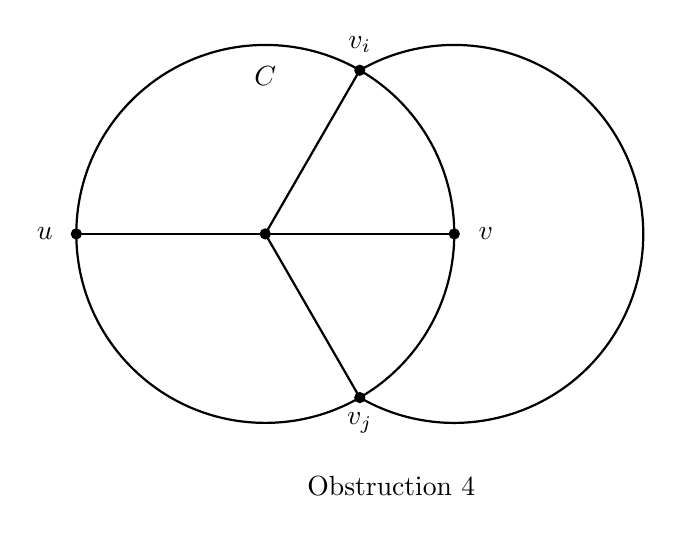
\begin{tikzpicture}[scale = 0.8]
                \draw[black, thick] (0,0) circle (3);
                \draw[black, thick] (1.5,-{sqrt(27/4)}) arc (-120:120:3);
                \draw[black, thick] (3,0) -- (-3,0);
                \draw[black, thick] (0,0) -- (1.5,{sqrt(27/4)});
                \draw[black, thick] (0,0) -- (1.5,-{sqrt(27/4)});
                \filldraw[black, thick] (-3,0) circle (2pt);
                \filldraw[black, thick] (3,0) circle (2pt);
                \filldraw[black, thick] (1.5,{sqrt(27/4)}) circle (2pt);
                \filldraw[black, thick] (1.5,-{sqrt(27/4)}) circle (2pt);
                \filldraw[black, thick] (0,0) circle (2pt);
                \node at (1.5,3,0) {$v_i$};
                \node at (1.5,-3,0) {$v_j$};
                \node at (-3.5,0,0) {$u$};
                \node at (3.5,0,0) {$v$};
                \node at (0,2.5,0) {$C$};

                \node at (2,-4,0) {Obstruction 4};
            \end{tikzpicture}
        \end{minipage}
        \hfill
        \begin{minipage}{0.4\textwidth}
            \begin{tikzpicture}[scale = 0.8]
                \draw[black, thick] (3,0) arc (acos(0.6):180-acos(0.6):5);
                \draw[black, thick] (0,0) circle (3);
                \draw[black, thick] (1.5,-{sqrt(27/4)}) arc (-120:120:3);
                \draw[black, thick] (3,0) -- (-3,0);
                \draw[black, thick] (0,0) -- (1.5,{sqrt(27/4)});
                \draw[black, thick] (0,0) -- (1.5,-{sqrt(27/4)});
                \filldraw[black, thick] (-3,0) circle (3pt);
                \filldraw[black, thick] (3,0) circle (3pt);
                \filldraw[black, thick] (1.5,{sqrt(27/4)}) circle (3pt);
                \filldraw[black, thick] (1.5,-{sqrt(27/4)}) circle (3pt);
                \filldraw[black, thick] (0,0) circle (3pt);
                \node at (1.5,3,0) {$v_i$};
                \node at (1.5,-3,0) {$v_j$};
                \node at (-3.5,0,0) {$u$};
                \node at (3.5,0,0) {$v$};
                \node at (0,2.5,0) {$C$};
                \node at (2,-4,0) {$G$ chứa một subdivision của $K_5$};

            \end{tikzpicture}
        \end{minipage}
    \end{figure}
    \begin{remark}
        $G$ luôn có một đồ thị con là  subdivision của $K_5$ hoặc $K_{3,3}$
    \end{remark}
    Kết quả của 4 trường hợp trên đều mâu thuẫn với giả thiết. Từ đây, ta kết luận rằng, không tồn tại đồ thị nào như $G$. Định lý được chứng minh.
\end{proof}
